

\section*{Results}

% Execution times:
% 17 days for FastSurfer
% 3-4 days for SynthMorph
% 10-12 hours for FreeSurfer whole brain segmentation
% 5-7 hours for FreeSUrfer nonlinear registration


The numerical uncertainty measured for the SynthMorph CNN model was lower than 
for Freesurfer recon-all (Fig.~\ref{sm_boxplot},
as measured both in the resampled images ($p < 10^{-6}$, two-tailed paired t-test) and in the warp fields ($p < 10^{-5}$) despite only the libmath libraries in FreeSurfer being instrumented in contrast to the entirety of SynthMorph. 
The number of significant bits in warp fields was computed as the average number of significant bits across the x,y and z components.
%Moreover, finding comparable numerical uncertainty in the warp fields as in the registered images confirms that the uncertainty is not simply noise originating from the image itself \TG{I think making this comment would require way more explanations for which we don't have space here}.
On average, out of 24 bits available, the SynthMorph resampled image had 19.56 significant bits while FreeSurfer recon-all's had only 13.43 significant bits; the SynthMorph warp field had 18.55 significant bits while FreeSurfer recon-all's had only 14.12 significant bits.
% \TG{Ines: check average values}. 
These important differences show a clear superiority of the CNN model compared to FreeSurfer recon-all in terms of numerical uncertainty. 
Moreover, we also observed a larger variability of the numerical uncertainty across subjects in FreeSurfer recon-all compared to SynthMorph. 

% Moreover, we observe that the numerical instability observed in the registered images is present within the warp field that performed the registration.
% This confirms that the instability is not simply noise originating from the image itself, but is being introduced by the task being performed.
% In fact, the theory that the noise is being introduced by the task of registration is further validated by the comparable numerical instability between registered images and warp fields.
% When observing SynthMorph, we see that it is numerical stable at inference time as evidenced by the high value of the mean significant bits across registered images and warp fields.
% In fact, SynthMorph has an average of 19.56 significant bits per voxel in a registered image and 18.55 significant bits per voxel in a warp field while FreeSurfer respectively had 13.43 and 14.12 significant bits.




% FS vs SM boxplot
% Comment on significant differences due to p value
% Warp field + registered image instability is compared (not just noise that is being picked up)
% Discuss variability between SM and FS
% Mention outliers quickly

The differences in average numerical uncertainty observed between FreeSurfer and SynthMorph were confirmed by visual inspection of the non-linearly registered images and warp fields (Fig.~\ref{tbl:table_of_figures}).
% \TG{Remove the "non-linearly registered image. Mean significant bits" labels from Fig.1.b}
% \TG{Add "Significant bits" under color bar, increase font size in color bar to match caption size}
% \TG{Ines: I'm thinking that this figure might be a bit busy, what do you think of removing the warp fields since we don't have anything really meaningful to mention about them?} 
% \TG{Don't forget to fix the cuts in the MRIs, they are not the same slices as for the registered images.}).
% \Ines{Ok I'll remove them in the paper and include them in the extended table in the appendix}
The numerical uncertainty in registered images was structurally consistent, with higher uncertainty in the gray matter and at the border of the brain than in the white matter, both for SynthMorph and for FreeSurfer recon-all. The numerical uncertainty in warp fields exhibited interesting structural patterns that would benefit from further investigation. 

The numerical uncertainty of FastSurfer segmentations was significantly lower than for FreeSurfer recon-all in 31 out of 35 brain regions (Fig.~\ref{fig:fastsurfer_boxplot},
% \TG{Trying to check what happened in the region where differences are not significant, I realized it's quite difficult to distinguish between blue and green dots. Maybe red dots would be more relevant for FastSurfer?}\TG{check number of subject in figure caption, it says 33 but it might be 32}, red stars),
with very substantial differences in some regions.
Here again, a larger variability was observed in FreeSurfer recon-all segmentations than in FastSurfer segmentations.
% \TG{I disagree with this sentence: variability is much larger for FreeSurfer than for FastSurfer. We shouldn't compare FreeSurfer non-linear registration to FreeSurfer segmentation. I would say ``Here again, a larger variability was observed in FreeSurfer recon-all segmentations than in FastSurfer segmentations.}.
Overall, FastSurfer averages a Sørensen-Dice score of 0.99 across all regions, while FreeSurfer is at 0.92.
The differences in Sørensen-Dice scores observed between FreeSurfer recon-all and FastSurfer were confirmed in local entropy maps (Fig.~\ref{tbl:entropy} where we visually noted a substantial discrepancy between both methods.
For FreeSurfer recon-all, clusters of non-zero entropy values were observed across the brain, whereas for FastSurfer non-zero entropy values were limited to scattered voxels. 
The entropy maps, in addition to visual inspection, confirm that, despite the relatively high average Sørensen-Dice scores,  FreeSurfer recon-all exhibited variability identifying the edges of subcortical structures, while FastSurfer remained certain in its segmentations.

% \TG{remove "ROI" from x-axis label. Move stars right before region names, color starts in red. Add thin, light-grey vertical lines to help match regions to data. Put "FreeSurfer / FastSurfer" caption on top of FreeSurfer figure and make its layout horizontal. Replace "FreeSurfer" by "FreeSurfer recon-all"}
% The minimum Sørensen-Dice score measured across pairs of Random Rounding samples for a given subject was on average 0.99 for FastSurfer vs 0.92 for FreeSurfer recon-all. Sørensen-Dice scores lower than 0.9 were observed in all regions for FreeSurfer recon-all and in no region for FastSurfer. Overall, the numerical uncertainty measured in FastSurfer segmentations was clearly lower than in FreeSurfer recon-all segmentations.

% \TG{show a subject with Dice < 0.9 for FreeSurfer}).

% In addition, we see that structural consistency across FreeSurfer and SynthMorph is maintained.
% Besides being able to visually identify anatomical components of the brain through the significance map, we see that in general across FreeSurfer and SynthMorph, white matter is more numerically stable while the grey matter near the edge of the brain suffers from a decrease in significance.
% However, when observing the FreeSurfer results, we see that there appear to be local areas of uncertainty that vary from subject to subject, but seem to consistently appear near the outer reaches of the brain.
% These areas of uncertainty might be areas that are especially difficult for FreeSurfer to register, but nonetheless warrant further investigation, much like the intriguing patterns observed in the significance maps for the warp fields.
% Table of figures
% There is structural consistency across FS and SM (white matter is stable grey matter less so) – edges are unstable
% Interesting there are local points in FS that are unstable
% Intriguing warp patterns that warrant more investigation
% Differences seen in boxplot generally are confirmed specifically




\newcommand{\addpic}[3]{
  % 1: subject
  % 2: tool
  % 3: image or warp field
  \includegraphics[width=\linewidth]{figures3/#2_#3/#1.eps}
}

\newcommand{\addimg}[3]{
  % 1: subject
  % 2: tool
  % 3: image or warp field
  \includegraphics[width=\linewidth]{figures3/#2_#3/#1_sigmap.eps}
}
\newcolumntype{M}[1]{>{\centering\arraybackslash}m{#1}}

%('sub-0027393', 5.374403595956109), X
% ('sub-0026196', 5.846457213878657),
% ('sub-0026044', 6.271014907991904),
% ('sub-0027174', 6.555800093688536), 
% ('sub-0027268', 7.098026186315213),
% ('sub-0027294', 7.978348288702006),
% ('sub-0026036', 8.491517084600082),
% ('sub-0026017', 8.918379766205852),
% ('sub-0025507', 8.99818740458033),
% ('sub-0025879', 9.087371203660338),
% ('sub-0025350', 9.36247095733503),
% ('sub-0025930', 9.60203884146283),
% ('sub-0027214', 9.887641061855172),
% ('sub-0025555', 10.335235132832166),
% ('sub-0025436', 10.684209656132898),
% ('sub-0025993', 10.769144760190507),
% ('sub-0026175', 10.81011759446143),
% ('sub-0025248', 11.260411153385373),
% ('sub-0025531', 11.853142548864518),
% ('sub-0025011', 12.412603668677889),
% ('sub-0027012', 12.97043457392254),
% ('sub-0027110', 13.201163426026728),
% ('sub-0025362', 13.558726142148151),
% ('sub-0025604', 15.005388508359077),
% ('sub-0027191', 15.241092108290513),
% ('sub-0003002', 17.73971650371412),
% ('sub-0026055', 18.331364768588333),
% ('sub-0025462', 23.0),
% ('sub-0025631', 23.0),
% ('sub-0025598', 23.0),
% ('sub-2842950', 23.0),
% ('sub-0027094', 23.0),
% ('sub-0025406', 23.0),
% ('sub-0027434', 23.0), X
% ('sub-0027236', 23.0)

% \vspace*{-1cm}
\begin{figure}[t]
  \centering
  \begin{subfigure}[b]{0.48\linewidth}
    \hspace*{-1cm}                                                           
    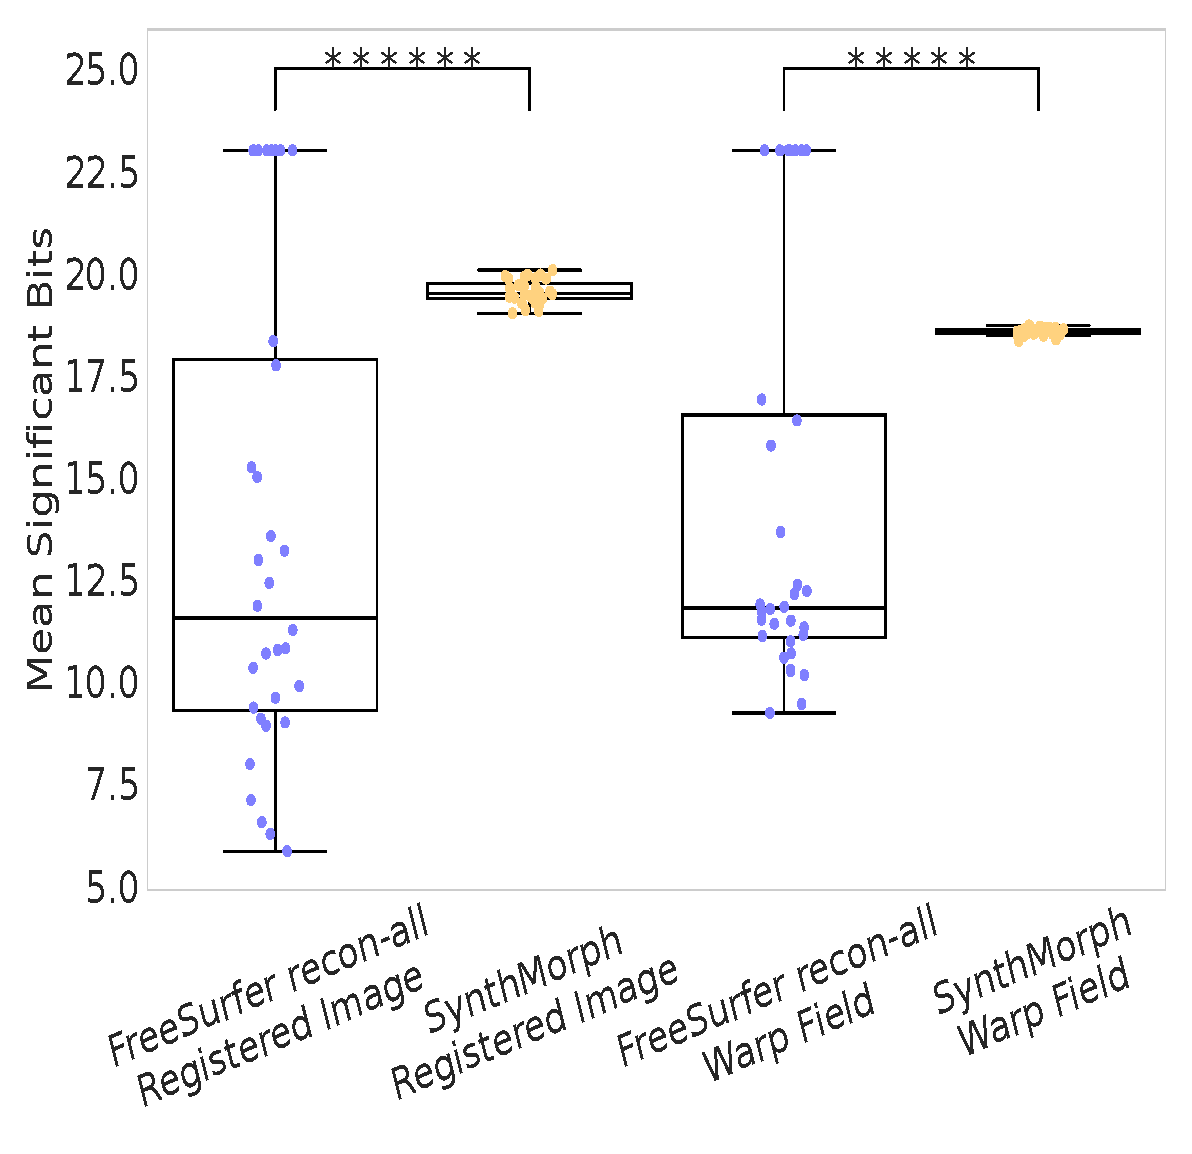
\includegraphics[width=1.25\linewidth]{figures3/fs_sm_boxplot.eps}
    \caption{Average numerical uncertainty for n=32 subjects. Each data point represents the voxel-wise mean number of significant bits computed across 10 Random Rounding samples.} 
    % \TG{Increase font size} \TG{Write "FreeSurfer recon-all" instead of "FreeSurfer" everywhere}
    \label{sm_boxplot}
  \end{subfigure}
  \hfill
  \hfill
  \begin{subfigure}[b]{0.48\linewidth}
    \centering
    % \vspace*{0.5cm}
  \begin{tabular}{c}
    % \toprule
        % \scriptsize{Linearly Registered MRI} \\ 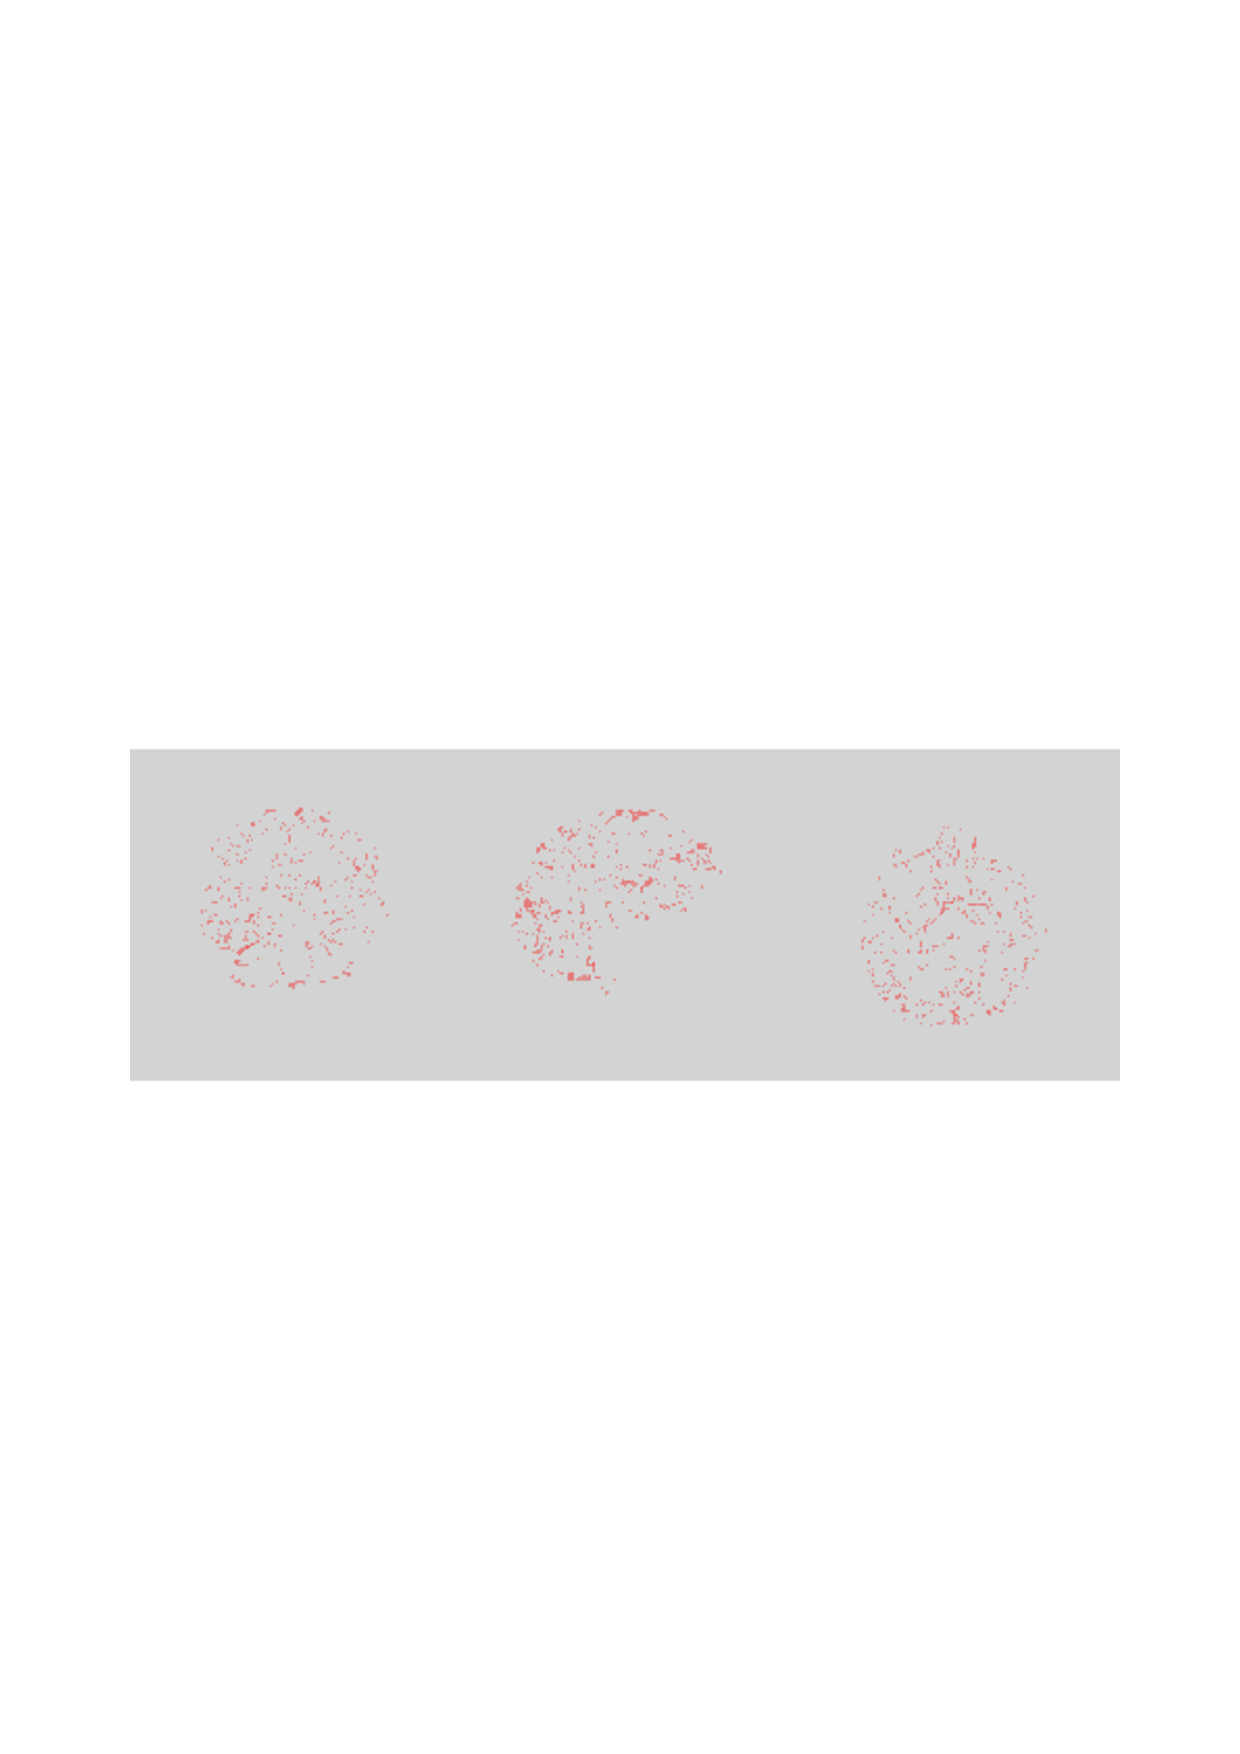
\includegraphics[width=12em]{figures3/linear_reg/sub-0025555.png} \\
        \includegraphics[width=\linewidth]{figures3/special_fig/fs_sub-0025555_sigmap.eps} \\
        % \addimg{sub-0025555}{fs}{reg} \\
        \scriptsize{FreeSurfer recon-all} \\
        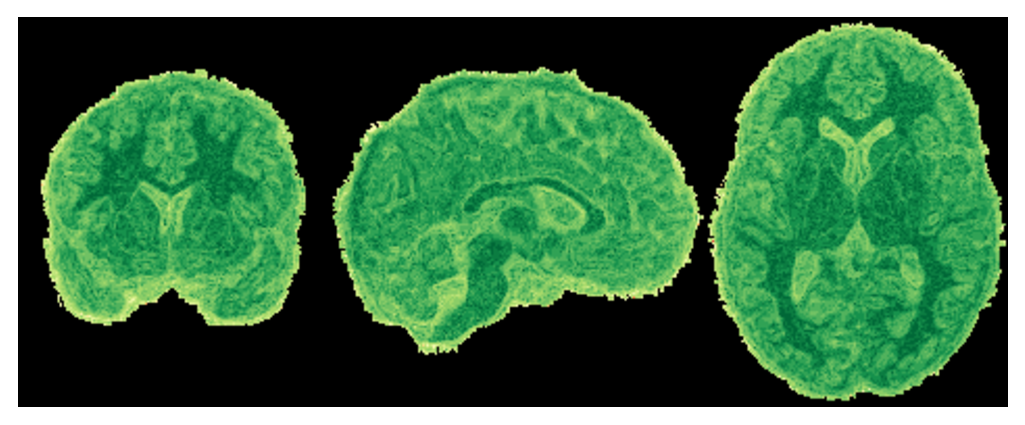
\includegraphics[width=\linewidth]{figures3/special_fig/sm_sub-0025555_sigmap.eps} \\
        % \addimg{sub-0025555}{sm}{reg} \\
        \scriptsize{SynthMorph} 
  \end{tabular}
  \centering
  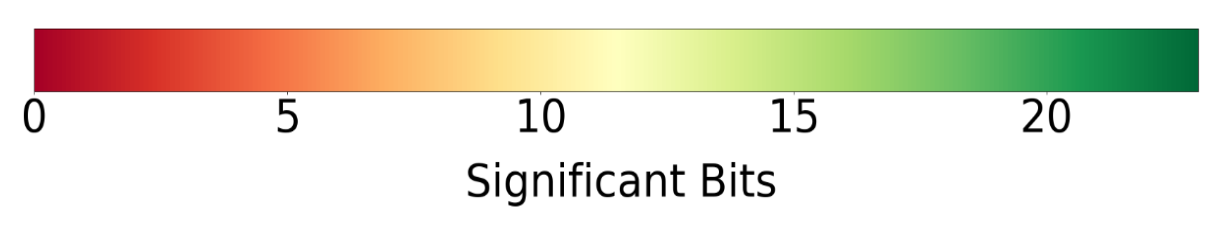
\includegraphics[width=\textwidth]{figures3/colorbar.eps}
  \caption{Uncertainty maps for sub-0025555. Uncertainty maps for all the subjects are reported in Appendix~\ref{appendix:non-linear-registration}. Due to required cropping of image dimensions for SynthMorph, the registered images do not have the same dimensions between SynthMorph and FreeSurfer.}
  \label{tbl:table_of_figures}
  \end{subfigure}
  \caption{Numerical uncertainty measured in the non-linearly registered images and warp fields produced by FreeSurfer recon-all and the SynthMorph CNN model. } 
  % \Yohan{Is it not Bits instead of Digits? If so, update the legends. Round the Mean Significant Bits value to 2 bits.} \TG{Increase font size}  \TG{Add caption to color bar} 
\vspace*{-0.5cm}                                                           

\end{figure}

\begin{figure}
  \centering
  \begin{subfigure}[b]{\linewidth}
    \hspace*{-1cm}                                                           
    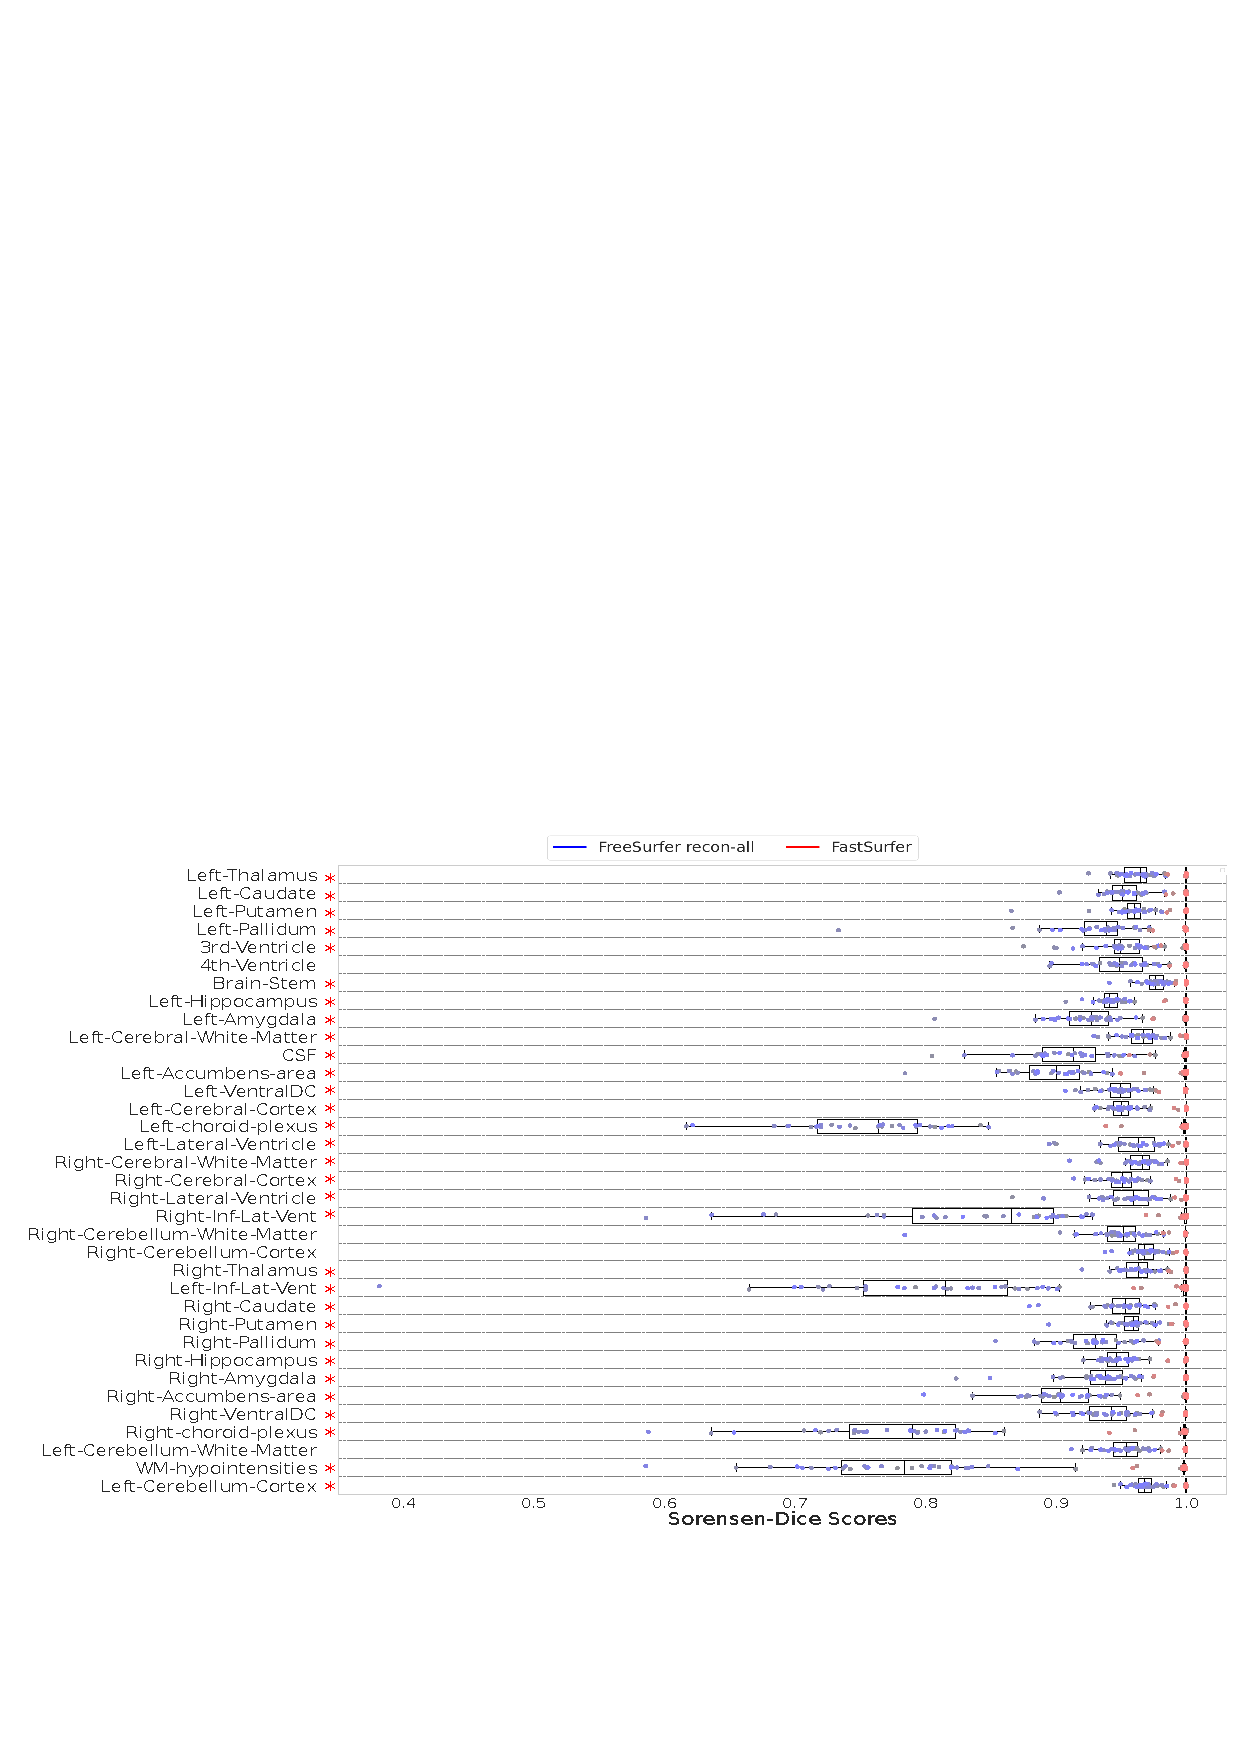
\includegraphics[width=1.25\textwidth]{figures2/fastsurfer_boxplot.pdf}
    \caption{Sørensen-Dice score comparison across FreeSurfer recon-all and FastSurfer for n=32 subjects. Each data point represents the minimum Sørensen-Dice score across all pairs of 5 Random Rounding samples for a given subject. \color{red}*\color{black}\xspace indicates significant differences between FastSurfer and FreeSurfer recon-all segmentations for the region ($p < 0.001$, two-tailed paired t-test with Bonferroni correction).} 
    \label{fig:fastsurfer_boxplot}
  \end{subfigure}
  \begin{subfigure}[b]{\linewidth}
    \centering
    \vspace*{0.5cm}
  \begin{tabular}{c c}
    % \toprule
        FreeSurfer recon-all & FastSurfer \\
        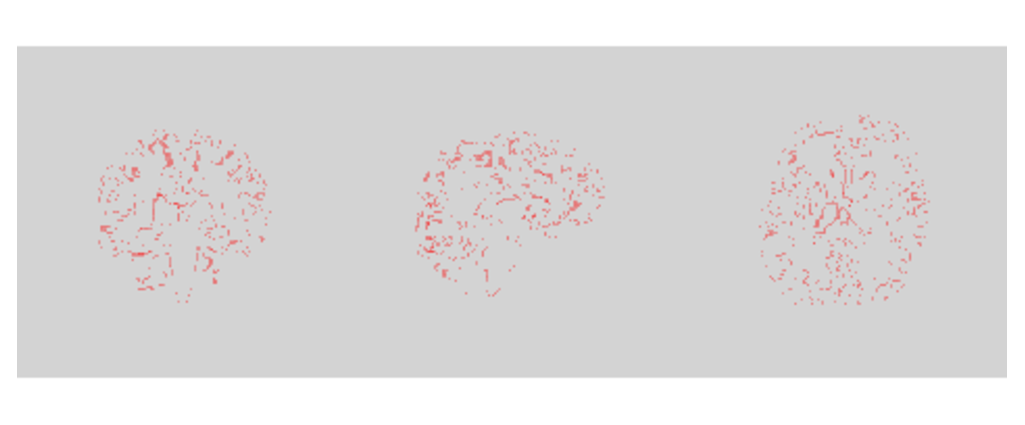
\includegraphics[width=0.5\linewidth]{figures3/special_fig/fs_sub-0027012_entropy.eps} & \includegraphics[width=0.5\linewidth]{figures3/special_fig/fast_sub-0027012_entropy.eps} \\
        % \scriptsize{FastSurfer} 
  \end{tabular}
  \centering
  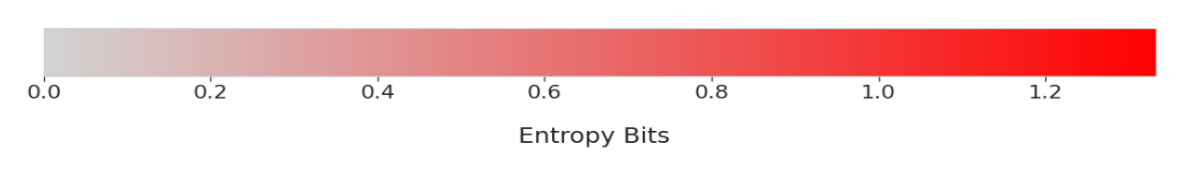
\includegraphics[width=0.6\textwidth]{figures3/entropy_colorbar.eps}
  \caption{Entropy maps for sub-0027012, computed across r=35 regions and n=5 Random Samples (see Eq.~\ref{eq:entropy}). Entropy maps for all the subjects are reported in Appendix~\ref{appendix:segmentation}.}
  \label{tbl:entropy}
  \end{subfigure}
  \caption{Numerical uncertainty measured in the segmentations produced by FreeSurfer recon-all and the FastSurfer CNN model. } 
\end{figure}